\documentclass[../main.tex]{subfiles}

\graphicspath{{../images/}}

\begin{document}
\pagestyle{fancy}
\lhead{Lecture 10: 2/15}
\chead{Chapter 7}
\rhead{PHYS 472}

\section*{Chapter 7: Energy Bands}
\addcontentsline{toc}{section}{Chapter 7: Energy Bands}

For a free electron, we know that the energy is quadratic i.e. $\epsilon \propto k^2$. We have a 
boundary condition for each states $2\pi/L$ and the energy is quantized. Some definitions
\begin{itemize}
    \item Metal: continous filled energy bands
    \item Insulator: an unfilled energy band
    \item Energy band gap $E_g$
    \item Metal: $E_g \to 0$
    \item Semi metal: $E_g < 0.4$ eV 
    \item Semi conductor: $E_g \approx 0.1 \to 4$ eV
    \item Insulator: $E_g > 4$ eV
\end{itemize}
insert book fig 2 chp 7
For the unperturbed case, we have a free electron with energy
\begin{align*}
    E_k = \frac{\hbar^2 k^2}{2m}(k_x^2 + k_y^2 + k_z^2), \qquad k_x, k_y, k_z = 0, \pm \frac{2\pi}{L}, \pm \frac{4\pi}{L}, \dots
\end{align*}
and wavefunction 
\begin{align*}
    \psi_k(\vb* \gamma) = e^{i \vb k \cdot \vb* \gamma}
\end{align*}
we have a plane wave with the Bragg condition
\begin{align*}
    (\vb k + \vb G)^2 = k^2 \implies k = \pm G/2
\end{align*}
where the $\vb G$ vector is the reciprocal lattice vector $\vb G = 2\pi/a$. The most scattered 
wave is $ k = \pm \pi/a$, and we get two solutions as a linear combination,
\begin{align*}
    \psi = e^{ikx} \pm e^{-ikx}
\end{align*}
We can substitute for when $k = \pm \pi/a$ for the standing waves and we get
\begin{align*}
    \psi(+) = 2 \cos(\frac{\pi}{a}x) \\
    \psi(-) = i2 \sin(\frac{\pi}{a}x)
\end{align*}
We can then define the corresponding probability density.
\begin{align*}
    \abs{\psi(+)}^2 \propto \cos^2(\frac{\pi}{a}x) \\
    \abs{\psi(-)}^2 \propto \sin^2(\frac{\pi}{a}x)
\end{align*}
insert book fig 3 chp 7

\newpage 
\lhead{Lecture 11: 2/20}

\section*{Chapter 7: Cont'd}
The first order energy difference is
\begin{align*}
    E_g &= \int_0^1 \dd x U(x) \qt[\abs{\psi(+)}^2 - \abs{\psi(-)}^2] \\
    &= 2 \int_0^1 \dd x U(x) \cos(\frac{2\pi}{a}x)
        \qt(\cos[2](\frac{2\pi}{a}x) - \sin[2](\frac{2\pi}{a}x)) \\
    &= U
\end{align*}
This is equal to the Fourier component of the crystal potential:
\begin{align*}
    U = U_o + U_1 \cos(\frac{2\pi}{a}x) + U_2 \cos(\frac{4\pi}{a}x) + \dots
\end{align*}

\paragraph*{Bloch Theorem} A constraint on the wavefunction as it is a periodic function:
\begin{align*}
    \psi_k(\vb r) = u_k(\vb r) e^{i\vb k \cdot \vb r}
\end{align*}
where $u(\vb r + na) = u(\vb r)$ is the periodic part of the wavefunction. $k$ is like a quantume
number where it represents the crystal momentum. 
\paragraph*{Simple proof:} (not accurate, take a look at Ashcroft and Mermin) Given a wavefunction
\begin{align*}
    \psi(x + a) = C \psi(x)
\end{align*}
where $a$ is the lattice constant and $C$ is a constant or eigenvalue in the formal case. The
\emph{Periodic boundary condition}(Born-Karman] we have a ring with $N$ lattice points so 
\begin{align*}
    \psi(x + Na) = \psi(x) \\
    C^N \psi(x) = \psi(x) \implies C^N = 1 \\
    \implies C = e^{i2\pi s/N}; \qquad s = 0, 1, 2, \dots, N-1 \\
    \implies \psi(x) = u_k(x) e^{i2\pi s x/Na}
\end{align*}
where \[\frac{2\pi}{a} \frac{s}{N}\] is the $k$ vector. So we don't need to solve the whole
equation, but rather just the periodic part $u_k(x)$. But true materials are not perfect crystals
or harmonic potentials, so we have to solve the Schrodinger (wave) equation for the crystal 
potential.
\begin{align*}
    m e^2 \tau / N1
\end{align*}
remember this???
\paragraph*{Kronig-Penney Model} We have a periodic finite potential well where 
the height of the potential is $U_o$, and in the region $0 < x < a$ we have a potential well
$U = 0$ and in the region $-b < x < 0$ we have a barrier $U = U_o$ that is periodic. From the 
wave equation:
\begin{align*}
    -\frac{\hbar^2}{2m} \dv[2]{\psi}{x} + U(x) \psi = \epsilon \psi
\end{align*}
where $\epsilon$ is the eigenenergy. For the first region:
\paragraph*{$0 < x < a$}, $U = 0$ the general solution is the linear combination
\begin{align*}
    \psi(x) = A e^{ikx} + B e^{-ikx}
\end{align*}
where the energy is only kinetic:
\begin{align*}
    \epsilon = \frac{\hbar^2 k^2}{2m}
\end{align*}
\paragraph*{$-b < x < 0$}, $U = U_o$ which is constant, which is renormalized::
\begin{align*}
    \psi(x) = C e^{Qx} + D e^{-Qx}
\end{align*}
where there is no $i$ in the exponent since the plane wave is not oscillatory, but decays.
\begin{align*}
    U_o - \epsilon = \frac{\hbar^2 Q^2}{2m}
\end{align*}
at the boundary $x = 0$, the wavefunction and the derivative must be continuous:
\begin{align*}
    A + B &= C + D \\
    ik(A - B) &= Q(C - D)
\end{align*}
Using Bloch's theorem, we know that each potential barrier is the same, but with a phase shift:
\begin{align*}
    \psi(a < x < a + b) = \psi(-b < x < 0) e^{ik(a+b)}
\end{align*}
we get the contiuity condition:
\begin{align*}
    Ae^{ika} + Be^{-ika} &= (Ce^{-Qb} + De^{Qb})e^{ik(a+b)} \\
    ik\qt[Ae^{ika} - Be^{-ika}] &= Q\qt[Ce^{-Qb} - De^{Qb}]e^{ik(a+b)}
\end{align*}
with four equations and four unknowns, we can solve for the energy eigenvalues. To solve for the
energy eigenvalues, we can use the determinant of the matrix of the coefficients of the equations.
\begin{align*}
    \begin{pmatrix}
        1 & 1 & -1 & -1 \\
        ik & -ik & -Q & Q \\
        e^{ika} & e^{-ika} & -e^{-Qb+ik(a+b)} & -e^{Qb + ik(a+b)} \\
        ik e^{ika} & -ik e^{-ika} & -Q e^{-Qb+ik(a+b)} & Q e^{Qb + ik(a+b)}
    \end{pmatrix}
\end{align*}
and the solution is
\begin{align*}
    \qt[\frac{Q^2 - K^2}{2Qk}] \sinh(Qb) \sin(Ka) + \cosh(Qb) \cos(ka) = \cos (k(a+b))
\end{align*}
we can simplify this equation for $b \to 0$, $U_o \to \infty$: so
\begin{align*}
    \frac{Q^2 \cdot ba}{2} = P
\end{align*}
where $Q \gg K$ and $Qb \ll 1$ from 
\begin{align*}
    U_o - \epsilon = \frac{\hbar^2 Q^2}{2m} \\
    Q = \sqrt{\frac{2m(U_o - \epsilon)}{\hbar^2}}
\end{align*}
thus 
\begin{align*}
    \frac{P}{Ka} \sin(Ka) + \cos(Ka) = \cos(ka)
\end{align*}
\newpage
The only allowed states are between $-1$ and $1$ since $\cos{ka}$ has a range of $-1$ to $1$. We 
can also think of this as a band structure where the allowed states are the energy bands and the
grey areas are the forbidden states.
\begin{figure}[ht]
    \centering
    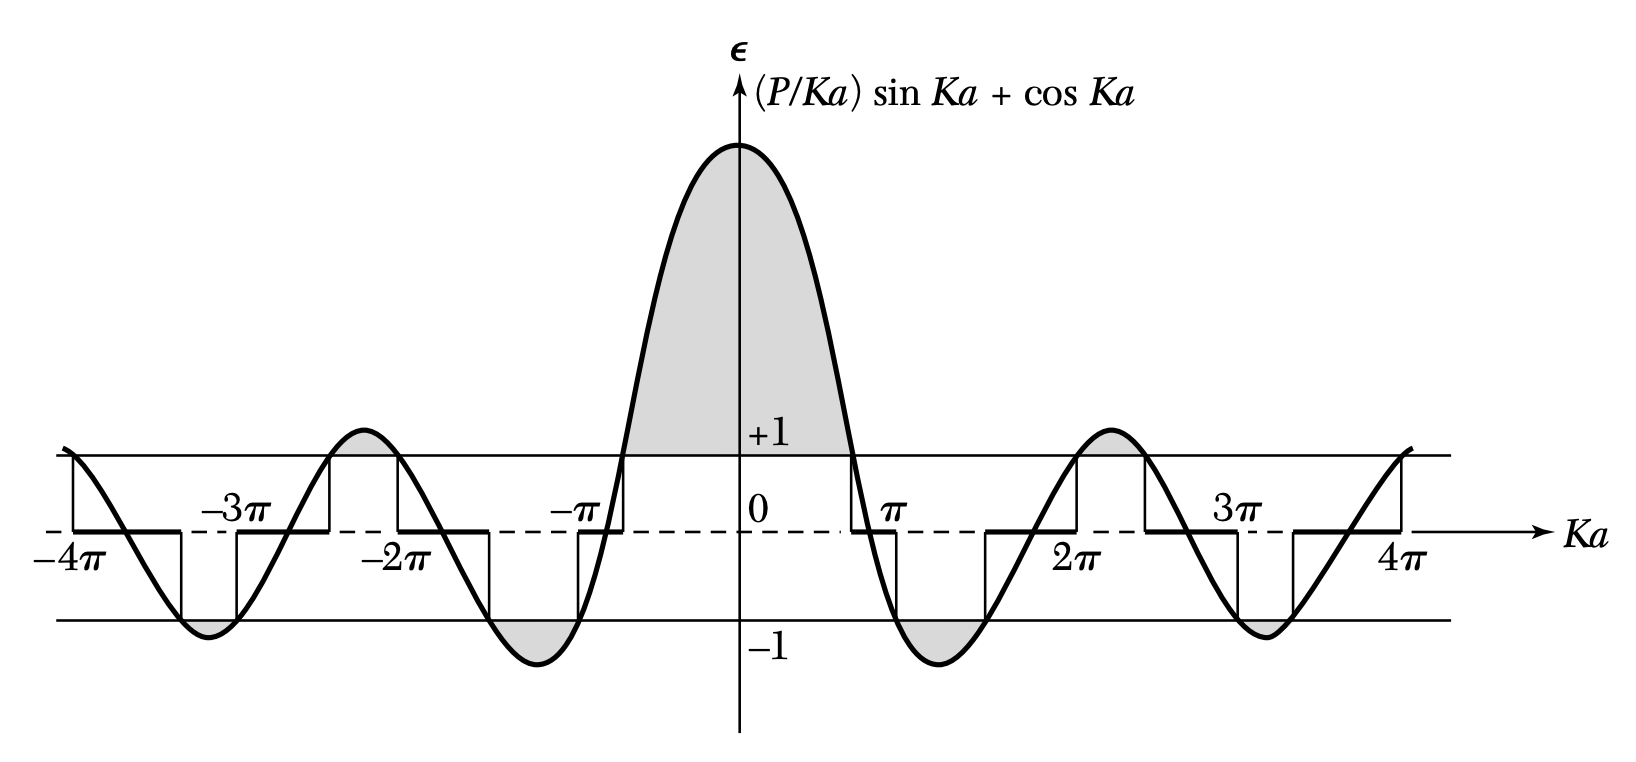
\includegraphics[width=0.6\linewidth]{kpmodel.png}
    \caption{The allowed states are where the $1 > \epsilon > 0$}
    \label{fig:7.1}
\end{figure}

\paragraph*{1D Case} from the Schr\"odinger equation for a periodic potential:
\begin{align*}
    -\frac{\hbar^2}{2m} \dv[2]{\psi}{x} + U(x) \psi = \epsilon \psi
\end{align*}
where $U(x + a) = U(x)$ is the periodic potential which can be expanded in a Fourier series:
\begin{align*}
    U(x) = \sum_G U_G e^{iGx}
\end{align*}
so 
\begin{align*}
    \qt(-\frac{\hbar^2}{2m} \dv[2]{\psi}{x} + \sum_G U_G e^{iGx}) \psi(x) = \epsilon \psi
\end{align*}
the wavefunction can be expanded in a Fourier series:
\begin{align*}
    \psi(x) = \sum_k C_k e^{ikx} \qquad k = \frac{2\pi n}{L}
\end{align*}
so we can substitute this into the Schr\"odinger equation:
\begin{align*}
    \qt[-\frac{\hbar^2}{2m} \dv[2]{\psi}{x}+ \sum_G U_G e^{iGx}] \sum_k C_k e^{ikx} = \epsilon \sum_k C_k e^{ikx} \\
    \frac{\hbar^2}{2m} \sum_k k^2 C_k e^{ikx} + \sum_{G, k} U_G C_k e^{i(k+G)x} = \epsilon \sum_k C_k e^{ikx}
\end{align*}

\newpage
\lhead{Lecture 12: 2/22}

\section*{Chapter 7: Cont'd}
From the single particle picture. The Schr EQ is
\begin{align*}
    \qt[-\frac{\hbar^2}{2m} \laplacian + U(\vb r)] \psi(x) = \epsilon \psi(x)
\end{align*}
where the potential is periodic:
\begin{align*}
    U(\vb r) = U(\vb r + \vb a)
\end{align*}
so the Fourier expansion of the solution
\begin{align*}
    \psi(x) = \sum_k C_k e^{ikx} ; \quad U(x) = \sum_G U_G e^{iGx}
\end{align*}
and subbing back in to the Schr EQ
\begin{align*}
    \sum_k \frac{\hbar^2 k^2}{2m} C_k e^{ikx} + \sum_{G, k} U_G C_k e^{i(k+G)x}
        = \epsilon \sum_k C_k e^{ikx}
\end{align*}
And since the reflected wave is $k' = k + G$, we can write the Schr EQ as
\begin{align*}
    \sum_k \qt[\frac{\hbar^2 k^2}{2m} + \sum_G C_{k-G} U_G e^{ikx}] = \epsilon \sum_k C_k e^{ikx} \\
    \frac{\hbar^2 k^2}{2m} + \sum_G C_{k-G} U_G = \epsilon C_k
\end{align*}
we define
\begin{align*}
    \lambda_k = \frac{\hbar^2 k^2}{2m} \\
    \implies (\lambda_k - \epsilon) C_k + \sum U_G C_{k-G} = 0
\end{align*}
which is the \emph{central equation} which can be solved for the energy eigenvalues. If we know the
wavefunction in 1D for a fixed $k$, the general formula for this wave function
\begin{align*}
    \psi_k(x) = \sum_G C_{k-G} e^{i(k-G)x}
\end{align*}
can satisfy the Bloch theorem i.e.
\begin{align*}
    \psi_k(x) = \sum_G C_{k-G} e^{-iGx} e^{ikx} = u_k(x) e^{ikx}
\end{align*}
where
\begin{align*}
    u_k(x + a) &= u_k(x) \\
    &= \sum_G C_{k-G} e^{-iG(x+a)} \\
    \qusing &G\cdot a = 2\pi n \implies e^{-iGx} = e^{-i2\pi n} = 1 \\
    &= \sum_G C_{k-G} e^{-iGx} = u_k(x)
\end{align*}
where the wave vector $k$ describes the crystal momentum.
\pagebreak
For a large oscillation, the kinetic energy (curvature) is large and the potential energy is small,
so the wavefunction is 
\begin{figure}[ht]
    \centering
    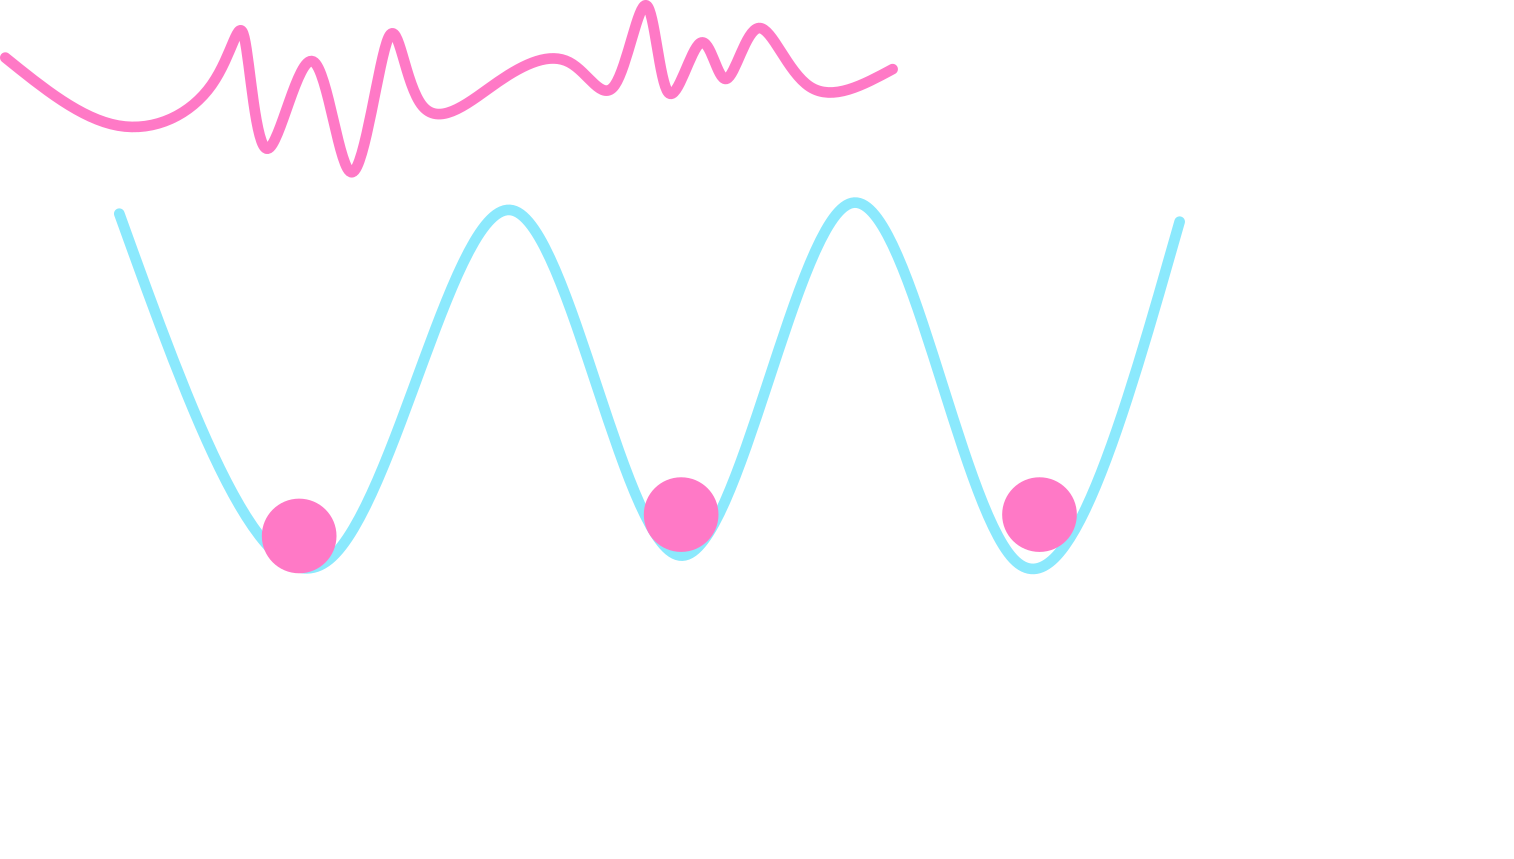
\includegraphics[width=0.6\linewidth]{wavefunctionish.png}
    \caption{For a small potential well, the wavefunction (in pink) has high curvature.}
    \label{fig:7.2}
\end{figure}

For Silicon the orbital configuration is $1s^2 2s^2 2p^2 3s^2 3p^2$ and the important valence
orbital is the $3s^2 3p^2$ where we denote $sp^3$ hybridization. There is a pseudo potential within
the core of the atom (Coulomb Potential) and the core electrons smooth out the potential AKA the 
pseudo potential approach. This is easier than the density functional theory (DFT) which is a

\paragraph*{Example:} Oversimplified case of a purely harmonic potential. THe $G$ vector as only
one component so $U(x) = U_G e^{iGx}$ where we fix $U_g = U_{-g} \neq 0$. For fixed $k$,
\begin{align*}
    \text{For } &k:\quad  (\lambda_k - \epsilon) C_k + U_g C_{k-g} + U_g + C_{k + g} = 0 \\
    &k-g; \quad (\lambda_{k-g} - \epsilon) C_{k-g} + U_g C_{k-2g} + U_g + C_{k} = 0 \\
    \vdots \\
    &k+g:
\end{align*}
from $k - 2g$ to $k + 2g$. The matrix is
\begin{align*}
    \begin{pmatrix}
        \ddots \\
        \dots & \lambda_{k - 2g} - \epsilon & U_g & 0 & 0 & 0 & \dots & e^{i(k-2g)x} \\
        & U & \lambda_{k-g} - \epsilon & U & 0 & 0 & \dots & e^{i(k-g)x} \\
        & 0 & U & \lambda_k - \epsilon & U & 0 & \dots & e^{ikx} \\
        & & & & & & \ddots
    \end{pmatrix}
\end{align*}
\paragraph*{Kronig-Penney Model in Reciprocal Space} Defining the potential barriers as a delta 
function, the new potential is
\begin{align*}
    U(x) = A \cdot a \sum_s \delta(x - sa) = \sum_G U_G \cos(Gx) \\
    = 2 \sum_{G>0} U_G \cos(Gx)
\end{align*}
where $A$ is a constant, $s$ is an integer, and $a$ is the lattice spacing. The Fourier transform
of $U_G$ is
\begin{align*}
    U_G = \int_0^1 \dd x U(x) \cos(Gx) = A
\end{align*}
Using the reciprotal lattice vector $G = 2\pi n/a$, we can write the central equation
\begin{align*}
    (\lambda_k - \epsilon) C_k + A \sum_n C_{k - 2\pi n/a} = 0
\end{align*}
to solve this, we define a function
\begin{align*}
    f(k) = \sum_n C_{k - 2\pi n/a} \implies f(k) = f(k - 2\pi m/a)
\end{align*}
so
\begin{align*}
    C_k = -\frac{\frac{2mA}{\hbar^2} f(k)}{k^2 - \frac{2m\epsilon}{\hbar^2}}
        \qquad \lambda_k = \frac{\hbar^2 k^2}{2m}
\end{align*}
and the shifted constant is
\begin{align*}
    C_{k-2\pi n/a} = -\frac{\frac{2mA}{\hbar^2} f(k)}{(k-2\pi n/a)^2 - \frac{2m\epsilon}{\hbar^2}} \\
    \implies f(k) = -\sum_n \frac{2m\frac{A}{\hbar^2} f(k)}{(k-2\pi n/a)^2 - \frac{2m\epsilon}{\hbar^2}}
\end{align*}
we can cancel the $f(k)$ and move the terms:
\begin{align*}
    \implies \frac{\hbar^2}{2mA} = -\sum_n \frac{1}{(k-2\pi n/a)^2 - \frac{2m\epsilon}{\hbar^2}}
\end{align*}
from the Kronig-Penney model, we defined the wave vector
\begin{align*}
    K^2 = \frac{2m\epsilon}{\hbar^2}
\end{align*}
so 
\begin{align*}
    \implies = - \sum_n \frac{1}{(k-2\pi n/a)^2 - K^2} = I
\end{align*}
using the very cool and interesting identity
\begin{align*}
    \cot(x) = \sum_n \frac{1}{\pi n + x}
\end{align*}
and the algebraic identity
\begin{align*}
    -\sum_n \frac{1}{A^2 - B^2} = \sum_n \frac{1}{A + B} \pm \sum_n \frac{1}{A - B}
\end{align*}
so
\begin{align*}
    I \implies \frac{a^2\sin(Ka)}{4Ka[\cos(ka) - \cos(Ka)]} \\
    \implies \frac{mAa^2}{2\hbar^2} \cdot \frac{1}{Ka} \sin(Ka) + \cos(Ka) = \cos(ka)
\end{align*}
 
\newpage
\lhead{Lecture 13: 2/27}
From the cental equation:
\begin{align*}
    (\lambda_k - \epsilon) C_k + \sum_G U_G C_{k-G} = 0
\end{align*}
where
\begin{align*}
    \epsilon = \frac{\hbar^2 k^2}{2m}
\end{align*}
where at the zone boundary $k = \pm \pi/a$, there is a strong resonance and the potential attenuates
dispersion. The reciprocal lattice vector is $G = 2\pi n/a$ and we have a dispersion relation at the
point $U(\pm G/2)$ or in other words
\begin{align*}
    U = U_{G/2} = U_{-G/2}
\end{align*} 
so we need to find the wave function at the zone boundary: A linear combination of the first 
boundary conditions
\begin{align*}
    \psi_k = C_{G/2} e^{iGx/2} + C_{-G/2} e^{-iGx/2}
\end{align*}
this gives the central equation
\begin{align*}
    \begin{cases}
        (\lambda - \epsilon)C_{G/2} + U C_{-G/2} = 0 \\
        (\lambda - \epsilon)C_{-G/2} + U C_{G/2} = 0
    \end{cases}
\end{align*}
where we can solve this eigenvalue problem by finding where the determinat is zero:
\begin{align*}
    \begin{vmatrix}
        \lambda - \epsilon & U \\
        U & \lambda - \epsilon
    \end{vmatrix} = 0
\end{align*}
The two solutions are
\begin{align*}
    \epsilon = \lambda \pm U = \frac{\hbar^2}{2m} (G/2)^2 \pm U \\
    \implies \epsilon_G \sim 2U
\end{align*}
so the wavefunction is
\begin{align*}
    \psi = e^{iGx/2} + e^{-iGx/2} = \begin{cases}
        \cos(Gx/2) \\
        \sin(Gx/2)
    \end{cases}
\end{align*}
the derivative of energy (slope) roughly relates to the velocity, and the curvatue
is proportional to the mass:
\begin{align*}
    \pdv[2]{(\frac{\hbar^2 k^2}{2m})}{k} \propto \frac{1}{m}
\end{align*}
so around $G/2$, $-G/2$ the wavefunction is
\begin{align*}
    \implies \psi(x) = C_k e^{ikx} + C_{k-g} e^{i(k-g)x}
\end{align*}
and we get a pair of central equations:
\begin{align*}
    \begin{cases}
        (\lambda_k - \epsilon) C_k + U C_{k-G} = 0 \\
        (\lambda_{k-G} - \epsilon) C_{k-G} + U C_k = 0
    \end{cases}
\end{align*}
and we solve the eigenvalues by finding the determinant resulting in the solutions:
\begin{align*}
    \epsilon = \frac{1}{2} (\lambda_{k-g} + \lambda_k) \pm \qt[\frac{1}{4}(\lambda_{k-g} = \lambda_k)^2 + U^2]^{1/2}
\end{align*}
we define the value
\begin{align*}
    K = k - \frac{G}{2} \qquad \abs{k} \ll 1
\end{align*}
so the dispersion relation is
\begin{align*}
    \epsilon_{k} &= \frac{\hbar^2}{2m} (G^2/4 + K^2) \pm \qt[4\lambda(\frac{\hbar^2K^2}{2m}) + U^2]^{1/2} \\
    &= \frac{\hbar^2}{2m} (G^2/4 + K^2) \pm \qt[1 + \frac{\lambda}{U^2} \frac{\hbar^2K^2}{2m} ]^{1/2} \\
    &= C \pm \frac{\hbar^2K^2}{2m} \qt[1 + \frac{2\lambda}{U}] \\
    &= \frac{\hbar^2K^2}{2m^*}
\end{align*}
where 
\begin{align*}
    m^* = \frac{mU}{\lambda}
\end{align*}
is the effective mass. So if the curvature is large, the effective mass is approaches zero. We want
the curvature to be smooth so the kinetic energy is large. Holes in semiconductors have a effective
mass. 
\paragraph*{Filling the Bands} Due to the Pauli exclusion principle, we can only occupy a finite
space within a band of energy. Each electron will occupy
\begin{align*}
    n = \frac{2\pi/a}{2\pi/N} = N
\end{align*}
$N$ is the number of unit cells... But there is spin degeneracy, so the electrons will actually occupy
\begin{align*}
    n = 2N
\end{align*}
So one band can hold 2 electrons from a unit cell. Silicon (fcc hexigonal holds 4 atoms )has 2 atoms(2 Primitive cells)
of valence 4, so we have 8 valence electrons filling the 4 bands in full hence an insulator. 
For alkali metals, the band is only half filled, and thus a metal:
\begin{itemize}
    \item Even number of electrons: insulator
    \item Odd number of electrons: metal
\end{itemize}
Gallium Arsenide (GaAs) is a semiconductor with a band gap of 1.4 eV. It is highly mobile structure,
and for example Gallium Nitride which has a band gap of 3.4 eV is used in blue LED's, as it can
carry higher voltage with less current(less heat). But its not used very much because it is hard to
grow. Compounds are harder to grow than elements, so it is more expensive than using Silicon. 
\end{document}